% \chapter{Wstęp}
\section{Zakres}
Praca obejmuje implementację sterownika, którego analizę możemy podzielić na:

\subsection{Baza danych}
\begin{itemize}
	\item Implementacja:
	\begin{itemize}
		\item \textit{std::vector<std::string, std::any>}
		\item Programowanie optymalne dla cache-u procesora
	\end{itemize}
	\item Klucz:
	\begin{itemize}
		\item Generowanie unikalnego;
		\item Walidacja - Extended \textit{POSIX Regexp}: ,,/[a-z]+\_[1-9]+'';
	\end{itemize}
	\item Operacje:
	\begin{itemize}
		\item Dodaj;
		\item Usuń;
		\item Aktualizuj;
		\item Pobierz wartość na podstawie : konkretnego/typu klucza;
	\end{itemize}
\end{itemize}
\begin{figure}[h!]
    \centering
    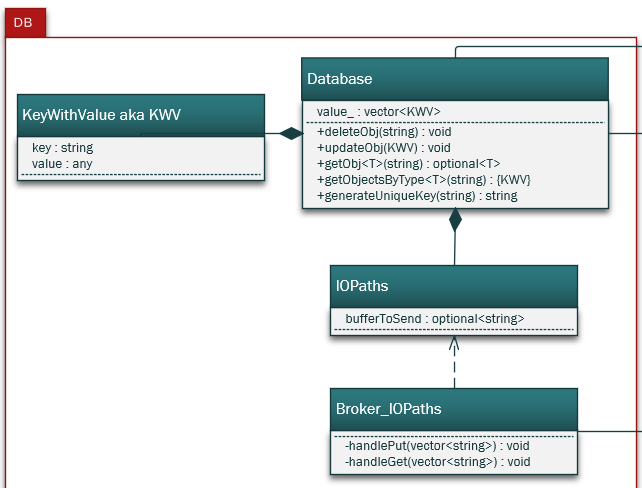
\includegraphics[scale=0.90]{Obrazki/DiagramyKlas/DB.png}
    \caption{Diagram klas przedstawiający relacje klas tworzących bazę danych.
        \newline(Opracowanie własne)}
\end{figure}

%%%%%%%%%%%%%%%%%%%%%%%%%%%%%%%%%%%%%%%%%%%%%%%%%%%%%%%%%%%%%%%%%%%%%%%%%%%%%%%%%%%%%%%%%%%%%%%%%%%%%%%%%%%%

\subsection{Back-end}
\begin{itemize}
	\item Realizacja wzorców projektowych:
	\begin{itemize}
		\item Komenda;
		\item Metoda szablonowa;
		\item Obiekt pusty;
		\item Budowniczy;
		\item \textit{RAII};
		\item Wstrzykiwanie zależności;
	\end{itemize}
	\item Implementacja:
	\begin{itemize}
		\item L1 - Warstwy fizycznej;
		\item L2 - Warstwy łącza danych;
		\item L7 - Warstwy aplikacyjnej;
	\end{itemize}
	\item Logowanie ruchu aplikacji:
	\begin{itemize}
		\item <h:min::s::ms> priorytet [nazwaPliku::nazwaFunkcji:numerLinii] komunikat;
		\item Obsługiwane priorytety: Trace < Debug < Info <  Warning < Error
		\item Filtrowanie w zależności od wybranego minimalnego priorytetu
		\item Rezultat przekazywany na wyjście standardowe oraz do pliku tekstowego
	\end{itemize}
\end{itemize}

%%%%%%%%%%%%%%%%%%%%%%%%%%%%%%%%%%%%%%%%%%%%%%%%%%%%%%%%%%%%%%%%%%%%%%%%%%%%%%%%%%%%%%%%%%%%%%%%%%%%%%%%%%%%

\subsection{Front-end}
\begin{itemize}
	\item Konsolowy interfejs użytkownika umożliwiający wydawanie komend do:
	\begin{itemize}
		\item Kontrolera sterownika;
		\item Bazy danych;
	\end{itemize}
	\item Realizacja wzorców projektowych:
	\begin{itemize}
		\item Komenda;
		\item Metoda szablonowa;
	\end{itemize}
	\item Przekazywanie logów aplikacji z Back-endu;
	\item Walidacja komend wpisanych przez użytkownika:
	\begin{itemize}
		\item Odrzucanie nieznanych komend;
		\item Podpowiedź odnośnie wartości argumentów komend już znanych;
	\end{itemize}
\end{itemize}

\begin{figure}[h!]
    \centering
    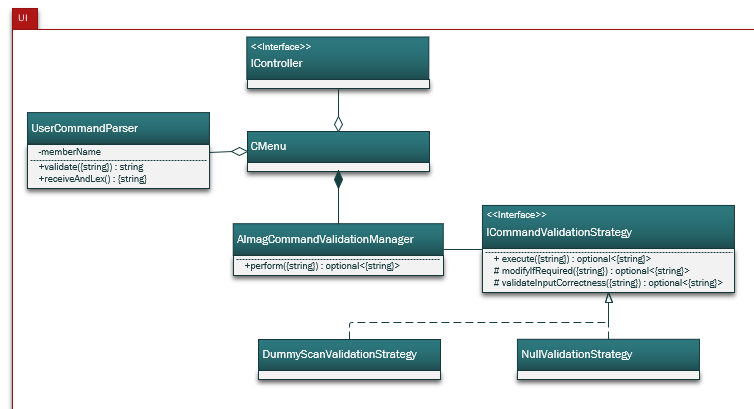
\includegraphics[scale=0.90]{Obrazki/DiagramyKlas/UI.png}
    \caption{Diagram klas przedstawiający klasy wchodzące w skład interfejsu użytkownika.
        \newline(Opracowanie własne)}
\end{figure}

%%%%%%%%%%%%%%%%%%%%%%%%%%%%%%%%%%%%%%%%%%%%%%%%%%%%%%%%%%%%%%%%%%%%%%%%%%%%%%%%%%%%%%%%%%%%%%%%%%%%%%%%%%%%

\subsection{Testowanie}
\begin{itemize}
\item Front-end
	\begin{itemize}
		\item Jednostkowe
		\item Modułowe
	\end{itemize}
\item Back-end
	\begin{itemize}
		\item Jednostkowe
		\begin{itemize}
			\item HDLC
			\item HDLC Body
			\item DB
		\end{itemize}
		\item Modułowe
		\begin{itemize}
			\item Happy Path
			\item Sad Path
		\end{itemize}
		\item Integracja
		\begin{itemize}
			\item UI + DB
			\item UI + DB + Back-end Controller
		\end{itemize}
	\end{itemize}
\item Komponentowe \newline
	W celu weryfikacji działania symulatora sterownika od początku do końca zalecane jest uruchomienie całego komponentu 
	jako czarną czarną skrzynkę oraz operowanie na nim przy pomocy zaimplementowanego interfejsu. W tym celu
	zaimplementowany został również symulator urządzenia, który odbiera wiadomości oraz odpowiada na nie.
\end{itemize}
